
%(BEGIN_QUESTION)
% Copyright 2015, Tony R. Kuphaldt, released under the Creative Commons Attribution License (v 1.0)
% This means you may do almost anything with this work of mine, so long as you give me proper credit

An SEL-487B differential current protective relay is used to provide protection for a three-terminal bus at an industrial facility substation:

$$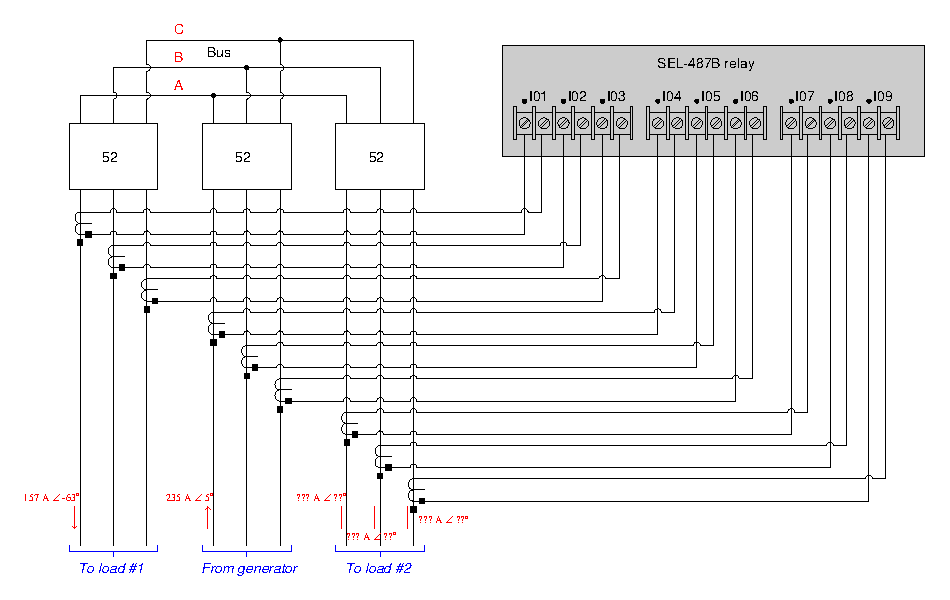
\includegraphics[width=15.5cm]{i02565x01.eps}$$

Calculate the magnitudes and phase angles for all three line currents feeding load \#2, assuming the generator and both loads are balanced, the bus is not faulted, and the phase rotation is ABC.  Be sure to place arrowheads on the current arrows for load \#2 in addition to expressing the currents in complex (polar) form. 

\underbar{file i02565}
%(END_QUESTION)





%(BEGIN_ANSWER)


%(END_ANSWER)





%(BEGIN_NOTES)

The arrowhead directions are arbitrary, but since the generator's phase A arrow is pointing upward (toward the substation bus) and load \#1's phase A arrow is pointing downward (away from the substation bus), it makes sense to sketch load \#2's phase A arrow downward as well.

With load \#2 phase A current arrow pointing down, we may apply Kirchhoff's Current Law to phase A at the substation bus.  The sum of the two currents exiting that node of the bus must equal the one current entering that node of the bus.  Therefore, for phase A:

$$I_{gen} = I_{load1} + I_{load2}$$

$$I_{load2} = I_{gen} - I_{load1}$$

$$I_{load2} = (235 \hbox{ A} \> \angle 5^o) - (157 \hbox{ A} \> \angle -63^o)$$

$$I_{load2} = 228.5 \hbox{ A} \> \angle 44.56^o$$

If the entire system is balanced (i.e. all phase and line quantities equal in magnitude with phase angles displaced by exactly 120 degrees), then the other two line currents for load \#2 must have the same magnitude but with different angles.  Given the ABC phase rotation, phase B's current must lag behind phase A by 120 degrees, while phase C's current must lag another 120 degrees (or lead phase A by 120 degrees):

$$I_{load2(A)} = 228.5 \hbox{ A} \> \angle 44.56^o$$

$$I_{load2(B)} = 228.5 \hbox{ A} \> \angle -75.44^o$$

$$I_{load2(C)} = 228.5 \hbox{ A} \> \angle 164.56^o$$


%INDEX% Electric power systems: protective relays (differential)
%INDEX% Electronics review: current transformer (CT)
%INDEX% Protective relay: differential current (87)

%(END_NOTES)


